\documentclass[a4paper,11pt,exos]{nsi} % COMPILE WITH DRAFT
\usepackage{pifont}
\usepackage{fontawesome5}
\usepackage{hyperref}



\begin{document}
\classe{\terminale Comp}
\titre{Corrigé de la préparat° à l'éval-bilan 4}
\maketitle






\dleft{11.5cm}{
    \exo{}
    Dans une kermesse, on fait tourner la roue de loterie équilibrée ci-contre où tous les secteurs ont le même angle.\\
    Le joueur gagne le nombre de points indiqué par le secteur désigné par la flèche.\\
    $X$ est la variable aléatoire qui donne le gain du joueur.
}
{
    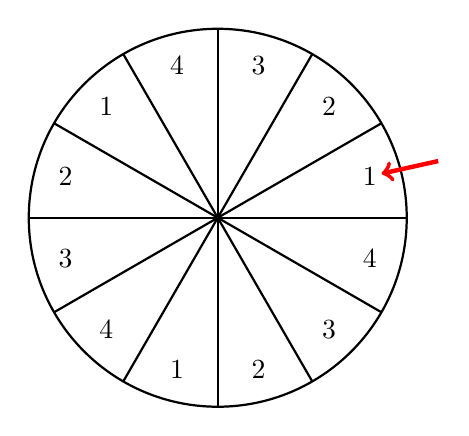
\begin{tikzpicture}[scale=.8]
        \foreach \i in {1,...,12} {
            \draw[thick] (0,0) -- ({30*\i}:3);
            %\node at ({30*(\i-0.5)}:2.5) {\i};
        }
        \foreach \i in {1,2,3,4} {
            \node at ({30*(\i-0.5)}:2.5) {\i};
            \node at ({30*(\i+3.5)}:2.5) {\i};
            \node at ({30*(\i+7.5)}:2.5) {\i};
        }
        \draw[thick] (0,0) circle(3);
        \draw[->, ultra thick, red] (3.5,.9) -- (2.6,.7); % Ajout de la flèche
    \end{tikzpicture}
}
\begin{enumerate}
    \item Quelle est la loi de probabilité suivie par $X$ ?
    \item Combien de points un joueur peut-il espérer gagner en moyenne lors d'une partie ?
    \item Pour pouvoir tourner la roue, le joueur doit payer 1 euro. Un point rapporte 0,40 €. Le jeu est-il équitable?
\end{enumerate}

\textcolor{UGLiBlue}{\textbf{Correction}
\begin{enumerate}
    \item $X$ suit une loi uniforme sur $\{1,2,3,4\}$.
    \item L'espérance de $X$ est $\dfrac{1+2+3+4}{4}=2,5$. Un joueur peut donc espérer gagner 2,5 points en moyenne lors d'une partie.
    \item Le joueur doit payer 1 euro pour jouer. Il peut espérer gagner $2,5\times 0,4$ € soit 1 €. Le jeu est donc équitable.
\end{enumerate}}


\exo{}
En janvier 2025, la ville de Rennes a subit une crue exceptionnelle de l'Ille. La précédente crue semblable a eu lieu en 1981.\\
On suppose que les crues de l'Ille sont indépendantes entre elles, qu'il y a au plus une crue par an et que chaque année, une crue se réalise avec une probabilité égale à 0,02.

\subsection*{Période entre deux crues}
Soit $T$ la variable aléatoire égale au nombre d'années écoulées avant la prochaine crue de l'Ille.\\ 
\textit{Si nécessaire, on arrondira les résultats à $10^{-4}$ près.}
\begin{enumerate}
    \item Calculer $P(T=1)$ et interpréter le résultat.
    \item Calculer la probabilité que la prochaine crue de l'Ille se produise dans 10 ans.
    \item Quelle est la loi de probabilité suivie par $T$ ? Préciser son (ou ses) paramètre(s).
    \item Justifier qu'une telle crue se produit en moyenne tous les 50 ans.
\end{enumerate}

\textcolor{UGLiBlue}{\textbf{Correction}
\begin{enumerate}
    \item $P(T=1)=0,02$. Cela signifie que la probabilité qu'une crue se produise l'année suivante est de 2\%.
    \item Pour que la prochaine crue de l'Ille se produise dans 10 ans, il faut qu'il n'y ait pas de crue pendant 9 ans puis une crue la 10$^\text{e}$ année.\\
    On a donc : $P(T= 10)=(1-0,02)^9\times 0,02\approx0,0167$.\\
    La probabilité que la prochaine crue de l'Ille se produise dans 10 ans est d'environ 1,67\%.
    \item La variable aléatoire $T$ modélise le temps pour obtenir un succès (ici une crue) en répétant de manière indépendante une expérience de Bernoulli de paramètre $p=0,02$.\\
    $T$ suit donc une loi géométrique de paramètre $p=0,02$.
    \item L'espérance d'une loi géométrique de paramètre $p$ est $\dfrac{1}{p}$.\\
    Donc $E(T)=\dfrac{1}{0,02}=50$.\\
    Une crue de l'Ille se produit donc en moyenne tous les 50 ans.
\end{enumerate}
}

\subsection*{Nombre de crues par siècle}
Soit $N$ la variable aléatoire égale au nombre de crues de l'Ille pendant les 100 prochaines années.
\begin{enumerate}
    \item Quelle est la loi de probabilité suivie par $N$ ? Préciser son (ou ses) paramètre(s).
    \item Calculer la probabilité qu'il n'y ait pas de crue de l'Ille pendant les 100 prochaines années.
    \item En déduire la probabilité qu'il y ait au moins une crue de l'Ille pendant les 100 prochaines années.
    \item À l'aide de la calculatrice, déterminer la probabilité qu'il y ait au moins 5 crues de l'Ille pendant les 100 prochaines années.
\end{enumerate}

\textcolor{UGLiBlue}{\textbf{Correction}
\begin{enumerate}
    \item La variable aléatoire $N$ compte le nombre de succès (ici le nombre de crues) en répétant 100 fois de manière indépendante une expérience de Bernoulli de paramètre $p=0,02$.\\
    $N$ suit donc une loi binomiale de paramètres $n=100$ et $p=0,02$.
    \item $P(N=0)=\binom{100}{0}\times 0,02^0\times 0,98^{100}\approx 0,1326$.\\
    La probabilité qu'il n'y ait pas de crue de l'Ille pendant les 100 prochaines années est d'environ 13,26\%.
    \item $P(N\geqslant 1)=1-P(N=0)\approx 0,8674$.\\
    La probabilité qu'il y ait au moins une crue de l'Ille pendant les 100 prochaines années est d'environ 86,74\%.
    \item $P(N\geqslant 5)=1-P(N<5)\approx 0,0508$.\\
    La probabilité qu'il y ait au moins 5 crues de l'Ille pendant les 100 prochaines années est d'environ 5,08\%.
\end{enumerate}
}

\exo{ Loi de refroidissement de Newton}
Une tasse de café est servie à une température initiale de 80°C. On la laisse refroidir dans une pièce à température ambiante de 20°C.\\
On va étudier à l'aide d'une suite le refroidissement du café en appliquant la loi de Newton.\\

Pour tout entier naturel $n$, on note $t_n$ la température du café (en °C)au bout de $n$ minutes.\\
On a ainsi $t_0=80$. Entre deux minutes consécutives $n$ et $n+1$, on a $t_{n+1}-t_n=-0,2(t_n-20)$.
\begin{enumerate}
    \item Conjecturer d'après le contexte le sens de variation de la suite $(t_n)$.
    \item Montrer que, pour tout entier naturel $n$, on a $t_{n+1}=0,8t_n+4$.
    \item Exprimer $t_n$ en fonction de $n$.
    \item Déterminer la limite de la suite $(t_n)$.
    %\item \faCalculator \hspace*{.2cm} Combien de temps faut-il pour que la température du café soit inférieure à 30°C ?
\end{enumerate}

\textcolor{UGLiBlue}{\textbf{Correction}
\begin{enumerate}
    \item On étudie le refroidissement d'un café. La température du café devrait donc diminuer et la suite $(t_n)$ devrait donc être décroissante.
    \item Soit $n$ un entier naturel.
    \begin{tabbing}
        $t_{n+1}$\=$=t_n-0,2(t_n-20)$\\
        \> $=t_n-0,2t_n+4$\\
        \> $=0,8t_n+4$.
    \end{tabbing}
    \item On a pour tout $n\in\N, t_{n+1}=0,8t_n+4$ et $t_0=80$.\\
    $(t_n)$ est une suite arithmétique de premier terme $t_0=80$ et de raison $q=0,8$.\\[.5em]
    \textbf{Suite constante vérifiant la relation de récurrence :} \begin{tabbing}
        Soit $x\in\R \qquad x=0,8x+4$\=$\Leftrightarrow x-0,8x=4$\\
        \>$\Leftrightarrow 0,2x=4$\\
        \>$\Leftrightarrow x=20$.
    \end{tabbing}
    La suite constante $(c_n)$ égale à 20 vérifie donc la relation $c_{n+1}=0,8c_n+4$ pour tout $n\in\N$.\\[.5em]
    \textbf{Suite géométrique auxiliaire :}\\[.5em]
    On définit la suite $(v_n)$ sur $\N$ par $v_n=t_n-c_n$.\\
    Montrons que $(v_n)$ est une suite géométrique :
    \begin{tabbing}
        Soit $n\in\N \qquad v_{n+1}$\=$=t_{n+1}-c_{n+1}$\\
        \> $=0,8t_n+4-(0,8c_n+4)$\\
        \> $=0,8t_n+4-0,8c_n-4$\\
        \> $=0,8(t_n-c_n)$\\
        \> $=0,8v_n$.
    \end{tabbing}
    $(v_n)$ est donc une suite géométrique de raison $q=0,8$ et de premier terme $v_0=t_0-c_0=80-20=60$.\\
    On a donc pour tout $n\in\N, v_n=v_0\times 0,8^n=60\times 0,8^n$.\\[.5em]
    \textbf{Terme général de la suite $(t_n)$ :}\\[.5em]
    On a donc pour tout $n\in\N, t_n=c_n+v_n=20+60\times 0,8^n$.\\
    \item $\lim\limits_{n\to+\infty}0,8^n=0$.\\[.5em]
    Donc $\lim\limits_{n\to+\infty} t_n=\lim\limits_{n\to+\infty}20+60\times 0,8^n=20$.\\[.5em]
    La température du café tend donc vers 20°C.
\end{enumerate}
}
\end{document}